\section{Nested variants}\label{sec:composition}

Section~\ref{sec:designspace} describes what a nested variant is in the engine: a sequence of primitives over a range of depths, sharing one leaf capacity, one node pool and one traversal. This appendix reports how such variants fared. The short answer is that they tie the best single structure wherever the hierarchy is in memory, and that they help only when the hierarchy itself is paged from a slow device without a cache, where pinning the hierarchy is several times faster still. Section~\ref{sec:discussion} summarises the result in one paragraph.

\begin{figure*}[tb]
\centering
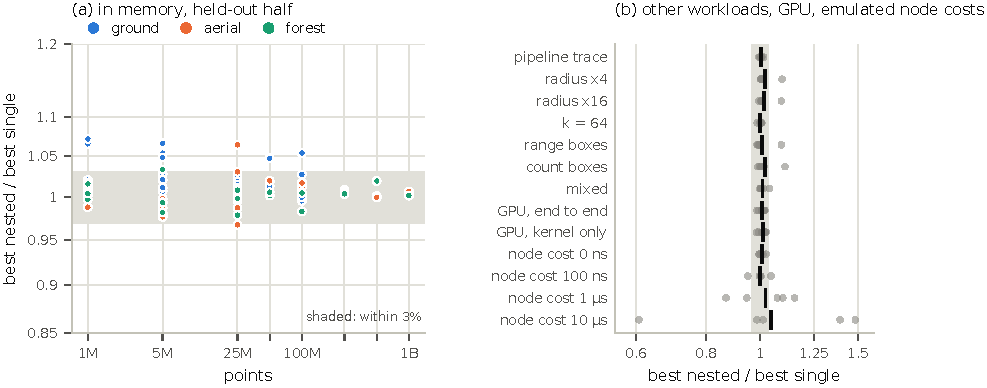
\includegraphics[width=\textwidth]{figures/fig_composition}
\caption{Best nested variant over best single structure. (a) The \nCells{} held-out clouds against their size, coloured by scan group; the band marks the 3\% tie zone. (b) The same ratio on seven workload variants of six 100M clouds, on the GPU for the normal-estimation pass of six clouds at two values of $k$, and under emulated per-node costs of 0 to 10\us{} on five 25M clouds; each dot is one cloud and the bar its geometric mean.}
\label{fig:composition}
\end{figure*}

\begin{table*}[t]
\centering\footnotesize
\caption{Nested variants in memory, held-out half, interleaved protocol: the best nested variant over the best single structure per cloud (geometric mean and range), wins, ties and losses at the 3\% band, the clouds in which the confirmation step adopted a nested variant, and the searched best over the fastest single timed on the held-out half.}
\label{tab:composition}
% generated by scripts/paper/tables.py; do not edit
\begin{tabular}{lrrrrrr}
\toprule
Cells & $n$ & nested picked & nested\,/\,single & range & wins\,/\,ties\,/\,losses & pick\,/\,oracle \\
\midrule
1M & 17 & 0 & 1.015 & 0.99--1.07 & 0\,/\,14\,/\,3 & 1.001 \\
5M & 16 & 0 & 1.013 & 0.98--1.07 & 0\,/\,11\,/\,5 & 1.002 \\
25M & 16 & 0 & 1.006 & 0.97--1.06 & 1\,/\,13\,/\,2 & 1.009 \\
50M & 6 & 0 & 1.017 & 1.00--1.05 & 0\,/\,5\,/\,1 & 1.000 \\
100M & 9 & 0 & 1.012 & 0.98--1.05 & 0\,/\,8\,/\,1 & 1.004 \\
250M & 3 & 0 & 1.006 & 1.00--1.01 & 0\,/\,3\,/\,0 & 1.001 \\
500M & 3 & 0 & 1.006 & 1.00--1.02 & 0\,/\,3\,/\,0 & 1.008 \\
1B & 3 & 0 & 1.004 & 1.00--1.01 & 0\,/\,3\,/\,0 & 1.000 \\
\midrule
ground & 31 & 0 & 1.020 & 0.98--1.07 & 0\,/\,24\,/\,7 & 1.004 \\
aerial & 25 & 0 & 1.005 & 0.97--1.06 & 1\,/\,21\,/\,3 & 1.004 \\
forest & 16 & 0 & 1.002 & 0.98--1.03 & 0\,/\,15\,/\,1 & 1.002 \\
\midrule
all & 73 & 0 & 1.011 & 0.97--1.07 & 1\,/\,60\,/\,12 & 1.003 \\
\bottomrule
\end{tabular}

\end{table*}

\begin{table}[t]
\centering\footnotesize
\caption{Nested variants in three other regimes: workload variants on the pipeline trace's centres (six 100M clouds), the GPU normal-estimation pass (six clouds, $k = 16$ and $32$; fastest of three rotated rounds), and an emulated cost added to every node a query enters (five 25M clouds, each cost with its own search). Below 1 the nested variant is faster.}
\label{tab:regimes}
% generated by scripts/paper/tables.py; do not edit
\begin{tabular}{lrrrr}
\toprule
Regime & $n$ & nested\,/\,single & range & picked \\
\midrule
workload base & 6 & 1.005 & 1.00--1.02 & -- \\
workload radius4 & 6 & 1.022 & 1.00--1.10 & -- \\
workload radius16 & 6 & 1.018 & 1.00--1.09 & -- \\
workload knn64 & 6 & 1.002 & 0.99--1.01 & -- \\
workload range8 & 6 & 1.010 & 0.99--1.09 & -- \\
workload count64 & 6 & 1.020 & 0.99--1.11 & -- \\
workload mixed & 6 & 1.011 & 1.00--1.04 & -- \\
\midrule
GPU, end to end & 12 & 1.010 & 0.99--1.02 & -- \\
GPU, kernel only & 12 & 1.013 & 0.99--1.03 & -- \\
\midrule
node cost 0 ns & 5 & 1.008 & 1.00--1.03 & 0 of 5 \\
node cost 100 ns & 5 & 1.000 & 0.95--1.05 & 1 of 5 \\
node cost 1 $\mu$s & 5 & 1.024 & 0.87--1.15 & 2 of 5 \\
node cost 10 $\mu$s & 5 & 1.046 & 0.61--1.48 & 1 of 5 \\
\bottomrule
\end{tabular}

\end{table}

\paragraph{In memory.} In none of the \nCells{} clouds did the confirmation step adopt a nested variant (Table~\ref{tab:composition}). The best nested variant is \nestedSingleAll$\times$ the best single over all clouds, between \nestedSingleLo{} and \nestedSingleHi{} in any one: \nestedTiesAll{} ties, \nestedLossesAll{} losses and \nestedWinsAll{} win at the 3\% band. The ratio does not move with size (Figure~\ref{fig:composition}a): \nestedSingleHundredM{} at 100 million points and \nestedSingleOneB{} at one billion. Timed sequentially on the nine 100M clouds (Table~\ref{tab:panelnested}), the best nested variant is \panelNestedSingleBase$\times$ the fastest single, at most \panelNestedSingleBaseMax{} in any cloud and never 3\% ahead; on 2\,MB pages nested and single variants gain alike. Nested variants build about eight percent faster with about six percent fewer nodes, because a wide prefix replaces several binary levels; neither buys query time.

\begin{table*}[t]
\centering\footnotesize
\caption{Nested variants in the headline panel at 100M points, sequential protocol, geometric mean (range, clouds). The out-of-core winners are the nested variants adopted with the hierarchy paged (below), timed in memory.}
\label{tab:panelnested}
% generated by scripts/paper/tables.py; do not edit
\begin{tabular}{lrr}
\toprule
Ratio & 4 KiB pages & 2 MB pages \\
\midrule
best nested / fastest single & 1.021 (1.00--1.05, $n$=9) & 1.032 (0.99--1.11, $n$=9) \\
out-of-core nested winner / searched best & 2.425 (2.17--2.79, $n$=3) & 2.514 (2.28--2.84, $n$=3) \\
\midrule
2 MB / 4 KiB pages, nested structures &  & 0.957 (0.92--0.99, $n$=12) \\
\bottomrule
\end{tabular}

\end{table*}

\paragraph{Other workloads, the GPU and expensive nodes.} Seven workload variants on the same centres (radii of four and sixteen times the trace's, $k = 64$, range boxes, count boxes and a mix) give the best nested variant \workloadNestedSingleMin{} to \workloadNestedSingleMax$\times$ the best single (Table~\ref{tab:regimes}). On an NVIDIA Quadro RTX 6000, with the same variants compiled into the same pool and queried by a warp-per-query kernel, it is \gpuNestedSingleTotal$\times$ end to end and \gpuNestedSingleKernel$\times$ in kernel time; a specialised GPU kd-tree, cudaKDTree~\cite{wald2022cudakdtree}, is \oursOverCudaKdTree$\times$ faster than any of our variants. Finally, an engine dial that makes a query spin for a fixed time on every node it enters, with a separate search per cost, moves the best nested over the best single from \nodeCostNestedSingleZero{} with no added cost to \nodeCostNestedSingleTenUs{} at 10\us{} per node: dearer nodes make nesting worse, not better, because what they call for is a larger leaf and a shallower tree, which a single structure provides directly.

\paragraph{Why the saved visits do not pay.} The best nested variants enter two to twenty percent fewer nodes than the best singles on the ground and forest scans. The visits they save are near the root, where a visit costs about \savedVisitCostNs\,ns because those levels stay in cache (Figure~\ref{fig:depth}); a leaf visit costs ten times more. On the aerial SanAndreas cloud the nested finalist, a quadtree over an octree, builds the same tree as the quadtree pick, because the octree levels never split height on flat terrain. Timed in different shuffled process groups, these two identical trees came out \nullPairMin{} to \nullPairMax{} apart, which is the noise of a variant-against-variant ratio under the interleaved protocol and the reason the headline ratios are re-timed sequentially.

\begin{table*}[t]
\centering\footnotesize
\caption{Out of core, modelled devices: the best nested prefix over each regime's best single, geometric mean and range over clouds, and the clouds in which a prefix was adopted (at least 3\% faster in every process). Hierarchy \emph{in RAM}: leaves on the device; \emph{paged}: the hierarchy read page by page as well.}
\label{tab:ooc}
% generated by scripts/paper/tables.py; do not edit
\begin{tabular}{lllllrl}
\toprule
Hierarchy & Cache & Workload & Device model & $n$ & best prefix\,/\,single & adopted \\
\midrule
in RAM & none & trace & SATA SSD & 5 & 0.982 (0.97--0.99) & none \\
in RAM & none & trace & HDD & 5 & 0.984 (0.97--0.99) & none \\
in RAM & none & trace & QLC SSD, at rest & 5 & 0.988 (0.98--0.99) & none \\
in RAM & none & boxes & SATA SSD & 4 & 0.991 (0.98--1.01) & none \\
in RAM & none & boxes & HDD & 4 & 1.979 (1.20--3.36) & none \\
in RAM & none & boxes & QLC SSD, at rest & 4 & 0.999 (1.00--1.01) & none \\
\midrule
paged & none & trace & SATA SSD & 5 & 1.023 (0.98--1.14) & none \\
paged & none & trace & HDD & 5 & 1.155 (1.00--1.21) & none \\
paged & none & trace & QLC SSD, at rest & 5 & 0.980 (0.86--1.10) & Lille 0.86, Waikato 0.96 \\
paged & 1\% LRU & trace & NVMe & 5 & 0.989 (0.98--1.00) & none \\
paged & 1\% LRU & trace & SATA SSD & 5 & 0.971 (0.92--1.00) & Lille 0.92, DomFountain 0.96 \\
\bottomrule
\end{tabular}

\end{table*}

\paragraph{Out of core.} The nested structures of Ogayar-Anguita et al.~\cite{ogayar2023nestedlidar} were measured in a store where every node was a file, and their gains were gains in node loads. With the leaf store of Section~\ref{sec:placement}, prefixes of two to eight quadtree, octree or grid levels were tried over each regime's best single, with the adoption rule of the search (Table~\ref{tab:ooc}). With the hierarchy in memory a prefix was adopted in \oocInRamAdopted{} of \oocInRamCells{} clouds, on every device class and workload. With the hierarchy paged it was adopted in \oocPagedAdopted{} of \oocPagedCells{}: a quadtree prefix over the kd-tree on two ground scans with a SATA-class device and a cache, and a two- or four-level quadtree over a hierarchical grid on two clouds of the QLC drive without a cache. The gain is all in hierarchy pages a binary tree would read. This is the regime of the 2023 study, and its result reproduces there: its nested variants run in \isprsOverLeafMatchedMin{} to \isprsOverLeafMatchedMax{} of the time of their leaf-matched, depth-capped singles, while a single tuned for the device is \isprsOverBestSingleMin{} to \isprsOverBestSingleMax$\times$ faster than they are. Keeping the \hierarchyMbMin{} to \hierarchyMbMax\,MB hierarchy in memory makes the best variant \pagedOverPinnedMinNoCache{} to \pagedOverPinnedMaxNoCache$\times$ faster than the best paged one without a cache, and the page-blocked node order of Section~\ref{sec:engine} removes most of the hierarchy reads that a prefix saves.

\paragraph{Why nesting looked good before.} Three things made nested hierarchies look faster than they are, and this study met all three before it controlled them. The singles they were compared with were at default parameters or under a depth cap: in an earlier battery of ours nested variants won on dense ground scans by up to a quarter, and the whole margin was a 22-level cap on the sliding-midpoint kd-tree, which a quadtree prefix lent the levels it was denied. The comparisons counted nodes, and the nodes a wide prefix removes are the cheap ones. And the one setting where the count is a cost, a hierarchy paged from a device without a cache, is one that pinning a few tens of megabytes avoids.
